\chapter{Конструкторский раздел}
\label{cha:design}

В этом разделе описан состав, структура и алгоритмы работы устройства отображения в виде конечных автоматов.

\section{Структура устройства отображения}

Структурная схема работы устройства отображения показана на рисунке \ref{fig:structure}.

\begin{figure}[ht]
    \centering
    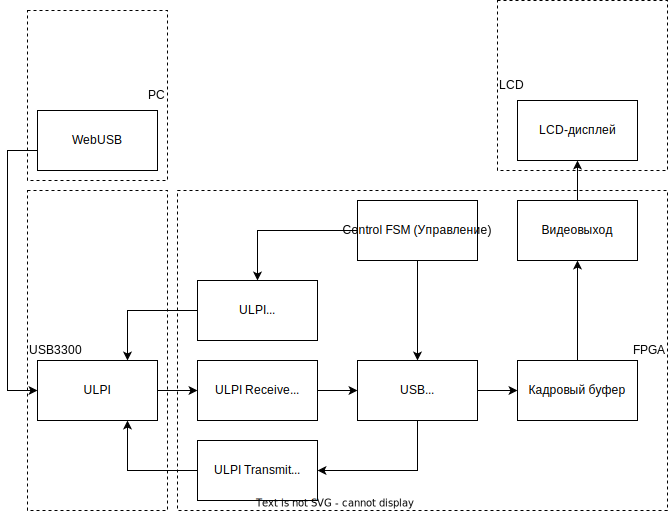
\includegraphics[scale=0.7]{res/img/structure.pdf}
    \caption{Структурная схема устройства отображения}
    \label{fig:structure}
\end{figure}

При запуске устройства происходит его инициализация. Затем ПК проводит опрос устройства, в ответ оно отправляет свои конфигурационные дескрипторы. После этого устройство считается сконфигурированным.

При помощи программы передачи изображения происходит отправка кадров устройству, сохраняющими их в кадровом буфере. Видеовыход вычитывает текущий кадр из буфера и отображает его на дисплее.

\section{Алгоритм работы устройства управления}

На рисунке \ref{fig:fsm_control_state} представлен конечный автомат блока управления. Устройство начинает с инициализации ULPI, после чего ожидает подключения USB интерфейса. Как только интерфейс будет сконфигурирован, блок управления будет ожидать отключения устройства. После отключения автомат вернётся в состояние ожидания подключения устройства.

\begin{figure}[ht]
    \centering
    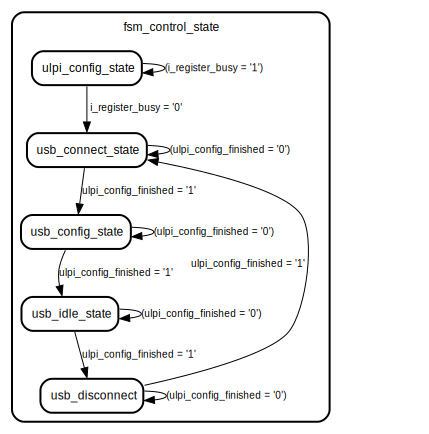
\includegraphics[scale=1]{res/img/fsm_control_state.pdf}
    \caption{Конечный автомат блока управления}
    \label{fig:fsm_control_state}
\end{figure}

\section{Алгоритм работы блока конфигурации}

Блок конфигурации обрабатывает сообщения протокола USB, поступающие от ПК, и формирует на них ответ. Его конечный автомат представлен на рисунке \ref{fig:fsm_usb_config_state}.

\begin{figure}[ht]
    \centering
    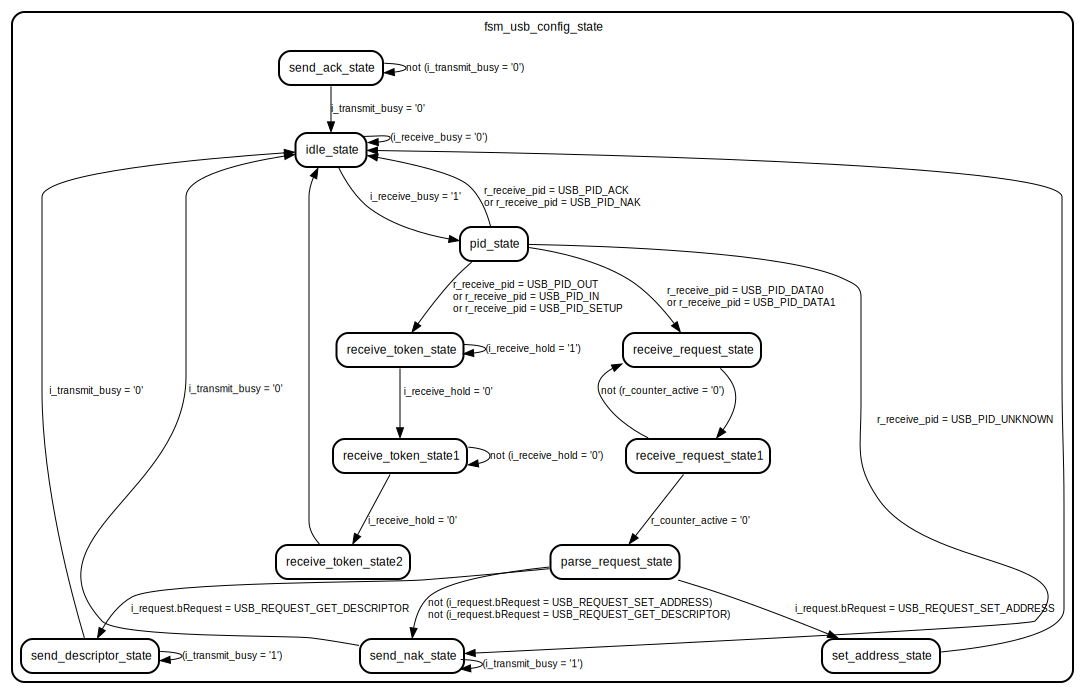
\includegraphics[scale=0.45]{res/img/fsm_usb_config_state.pdf}
    \caption{Конечный автомат блока конфигурации}
    \label{fig:fsm_usb_config_state}
\end{figure}

Конфигурация происходит в следующем порядке:

% \begin{enumerate}
\begin{enumerate}
\item ПК начинает транзакцию SETUP;
\item ПК запрашивает дескриптор устройства;
\item Устройство отвечает дескриптором;
\item ПК вновь начинает транзакцию SETUP;
\item ПК устанавливает адрес устройства;
\item Устройство принимает адрес и подтверждает;
\item ПК повторяет запрос дескриптора с новым адресом;
\item Устройство отправляет дескриптор;
\item ПК подтверждает принятие дескриптора и завершает транзакцию;
\item Устройство подтверждает завершение транзакции.
\end{enumerate}
% \end{enumerate}

\section{Алгоритм работы блока инициализации}

Блок инициализации записывает или считывает (в зависимости от команды) параметры из регистров ULPI. Его конечный автомат представлен на рисунке \ref{fig:fsm_ulpi_registers_state}.

\begin{figure}[ht]
    \centering
    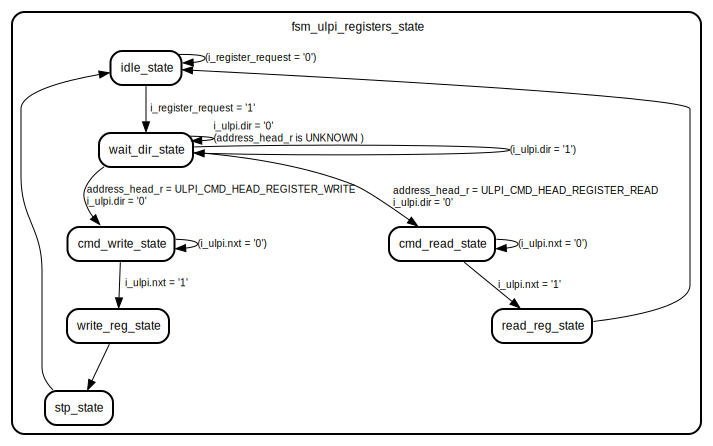
\includegraphics[scale=0.6]{res/img/fsm_ulpi_registers_state.pdf}
    \caption{Конечный автомат блока инициализации}
    \label{fig:fsm_ulpi_registers_state}
\end{figure}

\section{Выводы}

% \begin{enumerate}
\begin{enumerate}
\item Описана структура устройства отображения, выделены его составные части.
\item Описаны алгоритмы работы блоков в виде конечных автоматов.
\item Описан порядок конфигурации устройства в блоке конфигурации.
% \end{enumerate}
\end{enumerate}
